\documentclass[../main.tex]{subfiles}

\begin{document}
    \subsection{Komponenten des Aufbaus}
        Abbildung \ref{fig:Aufbau:Komponenten} zeigt alle Komponenten des Versuchs. Die Funktion der einzelnen Komponenten sind in \ref{fig:Aufbau:KomponentenErklaerung} erklärt. Der Nd:YAG-Laser wird hier optisch gepumpt durch eine Laserdiode, \textit{idealerweies} mit einer Wellenlänge von ca. $\SI{808}{\nano\metre}$, und produziert Licht mit einer Wellenlänge von ca. $\SI{1064}{\nano\metre}$.
        \begin{figure}[H]
            \centering
            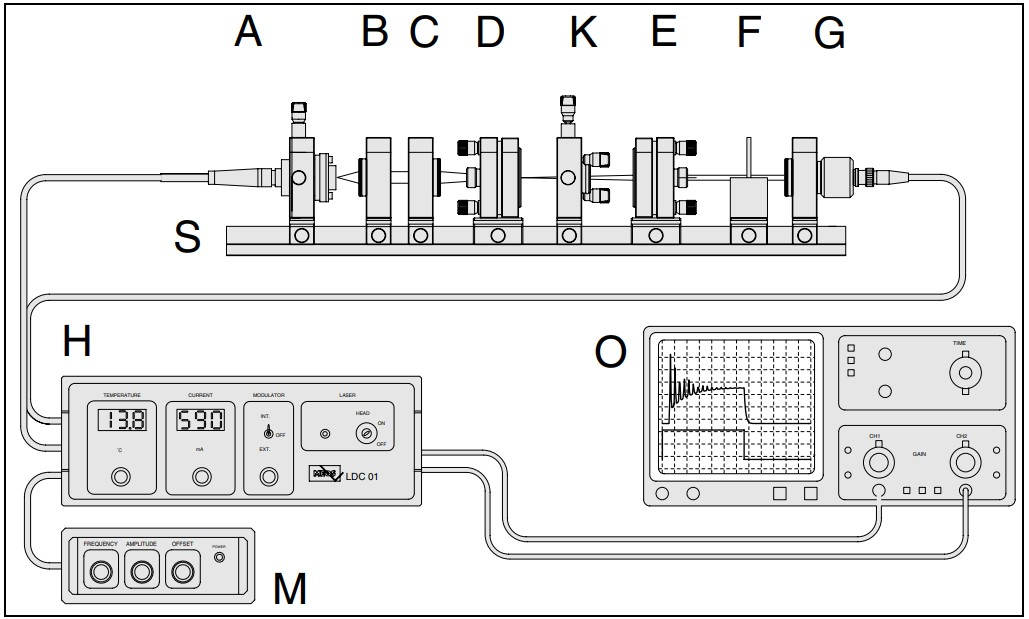
\includegraphics[width=0.8\textwidth]{Bilddateien/Versuchsaufbau/Komponenten.jpg}
            \caption{Komponenten zu Nd:YAG-Experimenten}
            \label{fig:Aubau:Komponenten}
        \end{figure}

        \begin{table}[H]
            \centering
            \begin{tabularx}{\textwidth}{cX}
                \textbf{Bezeichnung} & \textbf{Funktion}\\\hline\hline
                (A) & Diodenlaser zum Pumpen des Nd:YAG-Lasers.\\\hline
                (B) & Kollimator für Diodenlaserstrahl.\\\hline
                (C) & Fokussierlense für Diodenlaserstrahl ($f=\SI{60}{\milli\metre}$).\\\hline
                (D) & Modul, welches das aktive YAG-Medium enthält. An der rechten Seite des Mediums ist außerdem der rechte Resonatorspiegel (flach) angebracht. Das Modul besitzt außerdem Schrauben, mit welchen der Resonatorspiegel senkrecht zur optischen Axes des jeweiligen Aufbaus ausgerichtet werden kann. \\\hline
                (E) & Modul, das rechten Resonatorspiegel (Krümmungsradius $d=\SI{100}{\milli\metre}$) enthält. Auch hier sind Schrauben zur Justierung des Spiegel enthalten.\\\hline 
                (F) & Filterhalter mit zwei einsetzbaren Filtern: einen, um die Pumpwellenlänge zu blockieren, und einen, der nur die halbe Laserwellenlänge durchlässt.\\\hline
                (G) & Photodiode, Messung der Laserintensität?\\\hline
                (H) & Modul zur Steuerung des Injektionsstroms und der Temperatur der Laserdiode.\\\hline
                (K) & Kristall, in dem nichtlineare optische Effekte untersucht werden können.\\\hline
                (M) & Generator für periodische Injektionsströme in Modul H.\\\hline
                (O) & Oszilloskzop zur Messung des Injektionsstroms in Modul H und der Lichtleistung gemessen an Modul G.\\\hline
                (S) & Schiene zur Platzierung der Lasermodule.\\\hline
            \end{tabularx}
            \caption{Beschreibung der einzelnen Komponenten des Versuchaufbaus}
            \label{tab:Aufbau:KomponentenErklaerung}
        \end{table}

    

    \subsection{Anregungsspektrum des Nd:YAG-Kristalls}
        Um den Nd:YAG-Laser effizient betreiben zu können, wird zuerst untersucht, für welche Wellenlänge der Laserdiode die Pumpeffizient am höchsten ist, und wie sich die Wellenlänge der Laserdiode steuern lässt. Verwendet wird der in \ref{fig:Aufbau:Teil1} gezeigte Aufbau.  
        
        \begin{figure}[H]
            \centering
            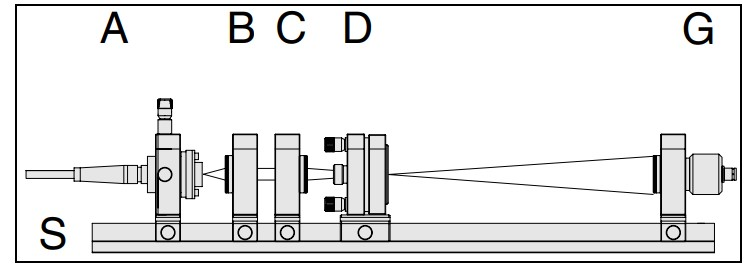
\includegraphics[width=0.8\textwidth]{Bilddateien/Versuchsaufbau/Teil1.jpg}
            \caption{Aufbau zur Untersuchung der Transmissionsrate des Nd:YAG-Kristall}
            \label{fig:Aufbau:Teil1}
        \end{figure}    

        \paragraph{Transmissionsspektren des Kristalls unter Diodenstrom.}\label{sec:Transmissionspektren}
        Zunächst wird ermittelt, für welche Wellenlänge der Laserdiode der YAG-Kristall minimale Transmissionsraten besitzt. Genau dort haben die Photonen der Laserdiode die passende Wellenlänge, um Anregung des Neodym\\
        
        % Die Besetzungsinversion der Laserdiode ist zwischen zwei Zuständen mit einer Bandlücke gegeben. Wie für Halbleiter üblich, ist die Breite dieser Bandlücke temperaturabhängig. Damit geht auch eine Abhängigkeit vom Injektionsstrom daher, welche einen Einfluss auf die Temperatur der Diode hat. Außerdem kann ein hoher Strom auch Übergänge in höhere Zustände bedingen, was zur Emission von Photonen mit kleinerer Wellenlänge führen kann. Um die Abhängigkeit der Diode von Injektionsstrom und Temperatur zu berücksichtigen, werden zwei Transmissionsspektren des Kristalls aufgenommen, aufgetragen über die Temperatur und bei je fixen Injektionsstrom $I_P=\SI{400}{\m\A}, \SI{550}{\m\A}$.

        \paragraph{Kennlinie für Konstante Wellenlänge.} Von den \textit{lokalen} Transmissionsmina eines der Transmissionsspektren wird nun das kleinste ausgewählt, da dort die meisten Zustände angeregt werden, die Pumpeffizienz also am größten ist. Assoziiert mit diesem Minima ist eine bestimmte Temperatur $T_{min}$, ein bestimmter Injektionsstrom $I_{min}$ und eine Pumpwellenlänge $\lambda_P^{(0)}$. Nun wird der Strom schrittweise variiert und für jeden Schritt die Temperatur bestimmt, für welche die Tranmissionrate des Kristalls wieder minimal ist. Der so erhaltene Zusammenhang $T_P(I_P)$ kann gefittet werden, wodurch sich eine kontinuierliche Kennlinie ergibt, entlang derer die Pumpwellenlänge $I_P$ konstant ist.\\
        
        Im weiteren Verlauf des Versuchs lässt sich immer wieder auf diese Kennlinie zurückgreifen: wenn ein bestimmter Strom $I_P$ oder eine bestimmte Temperatur $T_P$ eingestellt wird, liefert die Kennlinie die Temperatur $T_P'$ oder den Strom $I_P'$, sodass die Pumpwellenlänge gerade $\lambda_P$ ist.

    \subsection{Lebensdauer des $\,^4F_{3/2}$-Zustands}
        Als nächstes wird die Lebensdauer des angeregten $\,^4F_{3/2}$-Zustands für das Laserlicht bestimmt. Konkret ist das die Zeit $\tau$, in welcher \textit{durch spontane Emission} die Photonenzahl im $\,^4F_{3/2}$-Zustand auf das $1/e$-fache abgesunken ist. Je größer $\tau$ ist, desto leichter lässt sich eine Besetzungsinversion etablieren, $\tau$ ist also eine tatsächlich relevante Größe für die Charakterisierung eines Lasers.\\

        Der genutzte Versuchsaufbau ist in \ref{fig:Aufbau:Teil2} gezeigt. Hier dient das Filtermodul (F) zum Blockieren der Pumpwellenlänge $\lambda_P^{0}$, damit der Detektor G nur die durch spontane Emission im YAG-Kristall erzeugte Photonen misst.

        \begin{figure}[H]
            \centering
            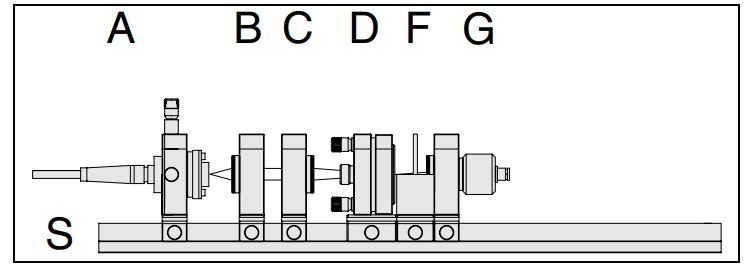
\includegraphics[width=0.8\textwidth]{Bilddateien/Versuchsaufbau/Teil2.jpg}
            \caption{Aufbau zur Untersuchung der Lebensdauer von $\,^4F_{3/2}$-Zuständen des Neodyms}
            \label{fig:Aufbau:Teil2}
        \end{figure}    

        Im Injektionsstromsgenerator (M) wird ein periodisches Rechteck-Signal angelegt. An dem an (G) gemessenen Signal sollte ein ebenso periodisch ein exponentieller Anstieg und ein exponentieller Abfall beobachtbar sein, aus dem die Lebensdauer $\tau$ berechnet werden kann.  

    \subsection{Aufbau des Nd:YAG-Kristalls.}
        Nun wird der zweite Resonatorspiegel (E) eingebaut, sodass ein funktionsfähiger Nd:YAG-Laser vorliegt (siehe \ref{fig:Aufbau:Teil4})

        \begin{figure}[H]
            \centering
            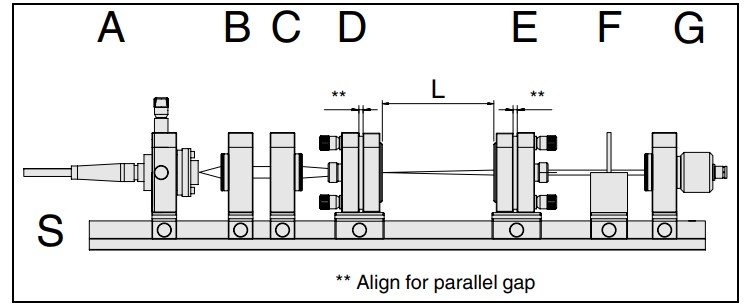
\includegraphics[width=0.8\textwidth]{Bilddateien/Versuchsaufbau/Teil4.jpg}
            \caption{Konstruktion des Nd:YAG-Lasers}
            \label{fig:Aufbau:Teil4}
        \end{figure}    

        Wichtig ist eine Wahl des Abstand $L$ derart, dass sich stabile Lichtmoden im zwischen beiden Resonatorspiegel ausbilden können. Für einen flachen und gekrümmten Spiegel (Krümmungsradius $R$, siehe \ref{tab:Aufbau:KomponentenErklaerung}) muss hierfür gelten 
        \[
            0\le 1 - \frac{L}{R}\le 1\implies 0\le L\le R.    
        \]

        Anschließend wird der Laser testeshalber in Betrieb genommen und die Resonatspiegel in (D), (E) mittels der Schrauben in den Modulen so ausgerichtet, dass die Laserleistung maximal wird. Weiterhin wird die Gelegenheit genutzt, die Transmissionsdiagramme aus Sektion \ref{sec:Transmissionspektren} zu bestätigen. Hierfür wird wieder bei $I_P = \SI{400}{\n\m}, \SI{550}{\n\m}$ die Laserleistung in Abhängigkeit von der Temperatur gemessen. Die Intervalle der gewählten Temperaturen sind gleich denen in \ref{sec:Transmissionspektren}. Da eine niedrige Transmissionrate des YAG-Kristalls eine hohe Pumpeffizienz des Lasers bedeutet, also eine große Laserleistung, sollten sich die hier aufgenommenen Diagramme genau invers zu denen aus \ref{sec:Transmissionspektren} verhalten.

    \subsection{Laserleistung als Funktion der Pumpleistung}
        

    \subsection{Laserausgangsleistung und Laserschwelle}

    \subsection{Spiking beim Laser-Einschaltvorgang}

    \subsection{Phänomene bei Frequenzverdopplung}
        \begin{figure}[H]
            \centering
            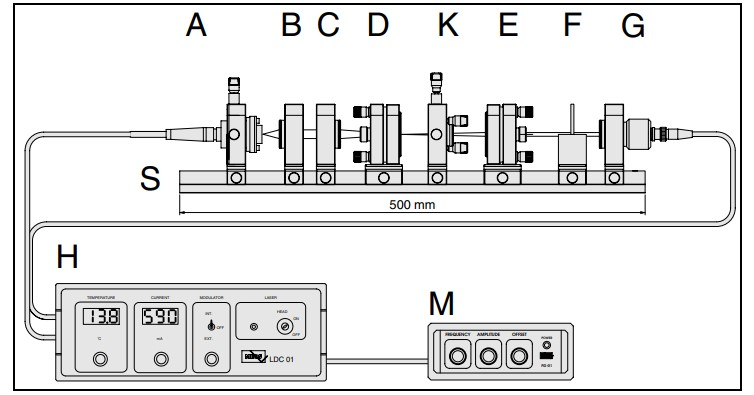
\includegraphics[width=0.8\textwidth]{Bilddateien/Versuchsaufbau/Teil7.jpg}
            \caption{Aufbau zur Untersuchung von nichtlinearen Effekten in Materie bei Bescheinung von Laserlicht}
            \label{fig:Aufbau:Teil7}
        \end{figure}    
        
        \paragraph{Lasermoden im Resonator.}
        
        \paragraph{Intensität des frequenzverdoppelten Lichts als Funktion der Pumpleistung.}

\end{document}